\noindent
\textbf{CHEM 352:
\ifthenelse{\equal{\solutions}{true}}{Examples}{Homework} for chapter 4.}\\

\noindent
1. Find all the possible symmetry operations for 1,2-propadiene:\\

\vspace{-0.5cm}
\begin{figure}[h]
\centering
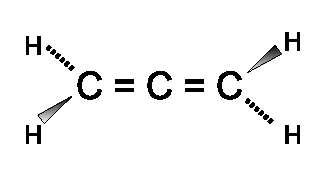
\includegraphics[scale=0.8]{allene}
\end{figure}
\vspace{-0.5cm}

\ifthenelse{\equal{\solutions}{true}}{% Problem 4/1 solution
\noindent
\underline{Solution:}\\

\noindent
The operations are: $E$, $C_2$, $C_2'$, $C_2''$, $S_4$, $S_4^3$, $\sigma_v$, $\sigma_v'$.\\
The $C_2$ axis is along C = C = C. The $C_2'$ and $C_2''$ axes are perpendicular to the $C_2$ axis
and are locate long the plane of the paper and perpendicular to the plane.\\

\hrule\vspace{0.5cm}



}{}

\noindent
2. Derive the $C_{2v}$ multiplication table by applying two successive symmetry operations
and identifying the resulting operation. Note that C$_{2v}$ point group is Abelian.\\

\noindent
\textbf{Note that you need to construct a multiplication table not a direct product table.}\\

\ifthenelse{\equal{\solutions}{true}}{% Problem 4/2 solution
\noindent
\underline{Solution:}\\

\noindent
The group is Abelian, which means that the order of multiplication does not matter, which simplifies the problem. The products can be worked out as follows:\\

\noindent
Multiplication by $OE$ (the identity operation) always yields $O$ as the result (where $O$ is one of the symmetry operations in $C_{2v}$).
Also operations such as $OO$ give $E$ (rotation and reflection). The only remaining operations are between $C_2$, $\sigma_v(xz)$ and $\sigma_v'(yz)$.
The molecule is taken to reside in $yz$ plane. 

\noindent
Let's consider $C_2\sigma_v$ as an example. To visualize what is happening, think about NO$_2$ molecul and place $p_x$ atomic orbitals on the oxygen
atoms. Note that the $x$ direction is out of the paper plane. $C_2$ will exchange the two oxygens and at the same time flip the $p_x$ orbitals around.
Then $\sigma_v$ reflection just exchanges the oxygens again but without flipping the $p_x$ orbitals. The net effect was to get flip the $p_x$ orbitals.
This same effect may be obtained by $\sigma_v'$ operation and therefore $C_2\sigma_v = \sigma_v'$. The same method can be used to go over all
the remaineng elements in the product table.\\

\hrule\vspace{0.5cm}



}{}

\noindent
3. What are the symmetry elements and point groups for the following molecules:\\

\vspace{-1cm}

\begin{figure}[h]
\centering
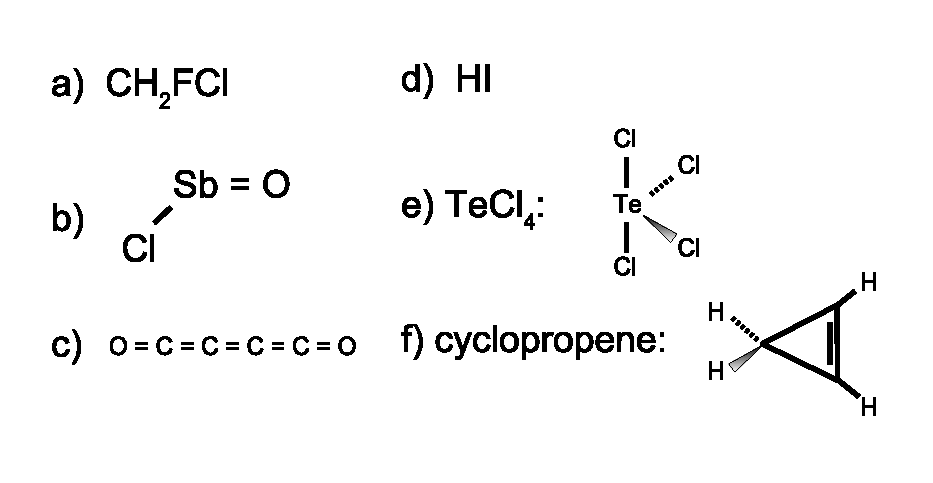
\includegraphics[scale=0.8]{molecules}
\end{figure}

\vspace{-1cm}

\ifthenelse{\equal{\solutions}{true}}{% Problem 3/4 solution
\noindent
\underline{Solution:}\\

Based on the lecture notes we have:

$$-\left(\frac{\partial S}{\partial P}\right)_T = \left(\frac{\partial V}{\partial T}\right)_P = \bar{V}\alpha \Rightarrow \Delta S \approx -\bar{V}\alpha\Delta P$$

Inserting the values into this equation we get:

$$\Delta S\approx -\frac{78.11\textnormal{ g mol}^{-1}}{0.879\textnormal{ g cm}^{-3}}\left(10^-2\textnormal{ m cm}^{-1}\right)^3\left(1.237\times 10^{-3}\textnormal{ K}^{-1}\right)\left(999\times 10^5\textnormal{ Pa}\right)$$
$$ = -10.99\textnormal{ J K}^{-1}\textnormal{ mol}^{-1}$$

\hrule\vspace{0.5cm}
}{}

\noindent
4. What are the irreps for $s$, $p$ and $d$ atomic orbitals in $D_{6h}$ point group?\\

\ifthenelse{\equal{\solutions}{true}}{% Problem 4/4 solution
\noindent
\underline{Solution:}\\

\noindent
From the character table we can see that both $x$ and $y$ correspond with the $E_{1u}$ irrep. The $p_x$ and $p_y$ orbitals
behave the same way and belong to $E_{1u}$ as well. By using the same logic, $p_z$ is $A_{2u}$. $s$ orbitals are always spherically
symmetric and hence this is $A_{1g}$. The Cartesian components of $d$ orbitals are: $d_{xz}, d_{yz}, d_{x^2 - y^2}, d_{xy}, d_{z^2}$.
These behave spatially exactly like the spatial operatiors (subscripts). As such. we immediately identify these as:
$E_{1g}$: $d_{xz}, d_{yz}$, $E_{2g}$: $d_{x^2-y^2}, d_{xy}$, and $A_{1g}$: $d_{z^2}$.\\


\hrule\vspace{0.5cm}



}{}

\noindent
5. The following are the normal vibration modes of water molecule:\\

\begin{figure}[h]
\centering
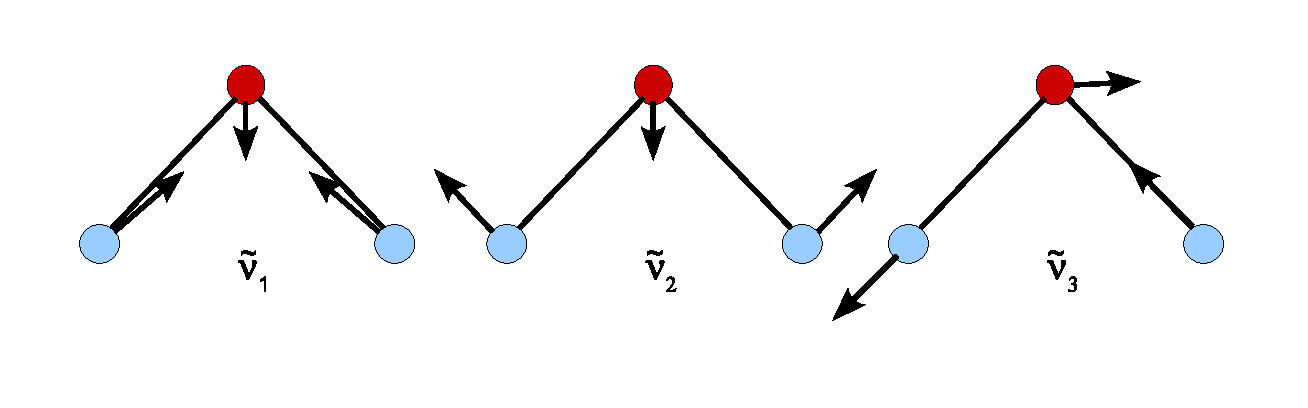
\includegraphics[scale=0.4]{water}
\end{figure}

\noindent
Apply the $C_{2v}$ symmetry operations for these modes and determine their irreducible representations
(consider the directionality of the vectors shown).

\ifthenelse{\equal{\solutions}{true}}{% Problem 4/5 solution
\noindent
\underline{Solution:}\\

\noindent
Mode 1 is unchanged under any symmetry operation in $C_{2v}$ and hence it has $A_1$ symmetry. The mode would be labelled as $a_1$.\\
Mode 2 is unchanged under any symmetry operation and hence the label is $a_1$.\\
The arrows correspond demonstrate the direction of atomic motion in molecular vibration.\\ 
Mode 3 is unchanged with $E$ and $\sigma_v'(yz)$ and the directions of the arrows get reversed ($-1$) with
$C_2$ and $\sigma_v(xz)$. Thus the mode is labelled as $b_2$.\\

\hrule\vspace{0.5cm}



}{}

\noindent
6. Consider H$_2$O molecule residing in $yz$ plane (symmetry $C_{2v}$). Let H$_1$ and H$_2$ denote their $1s$ orbitals. What are the irreps
for the following linear combinations: $S_1 = H_1 + H_2$ and $S_2 = H_1 - H_2$? Which oxygen atom valence orbitals
may form molecular otabitals with $S_1$ and $S_2$?\\

\ifthenelse{\equal{\solutions}{true}}{% Problem 4/6 solution
\noindent
\underline{Solution:}\\

\noindent
The orbitals $S_1$ and $S_2$ can be visualized as shown below (the first figure).
\begin{figure}[h]
\centering
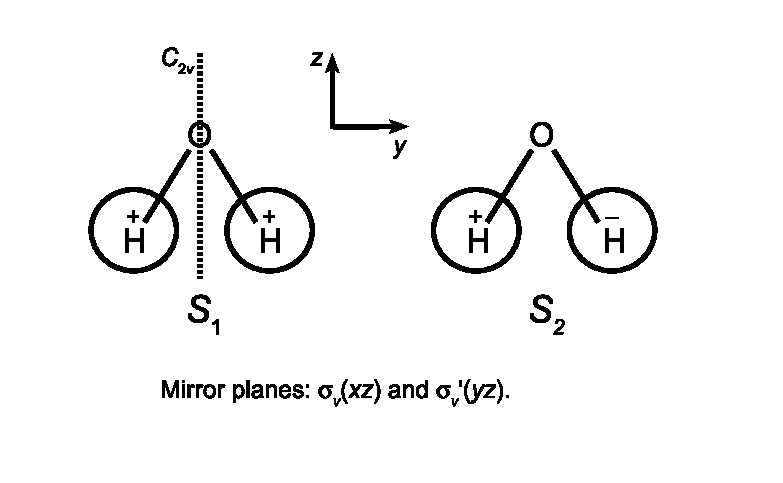
\includegraphics[scale=0.45]{watermo}
\caption{Visualization of $S_1$ and $S_2$ orbitals.}
\end{figure}
From this we can see that $S_1$ corresponds to $A_1$ (all operations give 1) and $S_2$ to $B_2$ (characters 1 $-1$ $-1$ 1).
The symmetry labels for the orbitals are therefore $a_1$ and $b_2$, respectively. The oxygen atom orbitals are shown in the second figure below.
\begin{figure}[h]
\centering
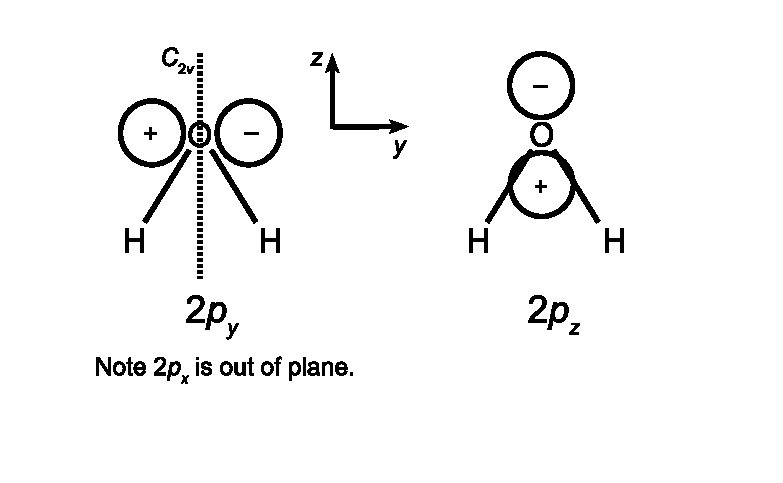
\includegraphics[scale=0.45]{watermo2}
\caption{Visualization of oxygen atom orbitals.}
\end{figure}
The $2s$ O orbital is clearly $A_1$ (totally symmetric). According to the above picture, $2p_z$ is also $A_1$. $p_y$ appears to
be $B_2$ and $p_x$ $B_1$. To find possible non-zero overlap integral value ($S$), we have to find pairs that produce $A_1$ when multiplied. Essentially, this says
that they must have the same symmetry. Thus $S_1$ can combine with $2s$ and $2p_z$ and $S_2$ with $2p_y$.\\

\hrule\vspace{0.5cm}



}{}

\noindent
7. Function $f_1$ exhibits symmetry corresponding to irrep $E_2$ and function $f_2$ irrep $A_1$ in $C_{6v}$ point group. Show that integral $\int f_1 x f_2d\tau = 0$ ($x$ represents multiplication by $x$ coordinate).\\

\ifthenelse{\equal{\solutions}{true}}{% Problem 7/4 solution
\noindent
\underline{Solution:}\\

\begin{itemize}
\item[a)] Use the following equation (see lecture notes):

$$\Delta G_2 = RT\ln\left(\frac{P_2}{P_1}\right) = (8.314\textnormal{ J K}^{-1}\textnormal{ mol}^{-1})\times (298.15\textnormal{ K})\times\ln\left(\frac{0.1\textnormal{ bar}}{1\textnormal{ bar}}\right)$$
$$ = -5.708\textnormal{ kJ mol}^{-1}$$

\item[b)] Gibbs energy is a state function and depends only on the endpoints. Thus the answer is the same as in a).

\end{itemize}

\hrule\vspace{0.5cm}
}{}

\noindent
8. The the ground state electronic wavefunction in H$_2$O has $A_1$ symmetry in $C_{2v}$ point group. What the symmetries
of the excited states that can absorb liearly polarized light in a) $x$, b) $y$ and c) $z$ directions?\\

\ifthenelse{\equal{\solutions}{true}}{% Problem 4/8 solution
\noindent
\underline{Solution:}\\

\noindent
The $C_2$ axis is along the $z$ axis and the molecule is in the $yz$ plane. The operator $x$ belongs to $B_1$. The ground state
is $A_1$ and by looking at the product table, we can see that the excited state must have $B_1$ symmetry ($B_1\times B_1 = A_1$).
For $y$ ($B_2$) and $z$ ($A_1$) the corresponding excited state symmetries must be $B_2$ and $A_1$, respectively.\\

\hrule\vspace{0.5cm}
}{}
